\chapter{Background} \label{ch:background}

Detailed description of many things. Blurb - brief description of cheminformatics, applications of computational tools to drug discovery. Maybe introduce design-make-teset? This stuff is probably in the introduction.

\section{Molecular Representation}

\subsection{SMILES}
The simplified molecular-input line-entry system (SMILES)  \cite{Weininger1988, Weininger1989} is a widely-used text-based description of molecular structure (Table~\ref{table:smiles}). In SMILES strings, atoms are represented with their chemical symbols and aromatic atoms are denoted in lowercase. Single and aromatic bonds are omitted while for double and triple bonds the specials characters \texttt{=} and \texttt{\#} are used. Branches are specified by enclosing them into parentheses. To encode cyclic structures a single bond in the ring is broken and the matching atoms are denoted by numbers. \texttt{@} characters are used to denote chirality while \texttt{\textbackslash} and \texttt{/} characters specify local double bond configurations. Following these rules, a SMILES string is constructed by traversing the nodes of the molecular graph. Depending on the choice of starting node and traversal route there are often multiple valid SMILES representations per molecule, especially for larger molecules. In order to define a single unique SMILES representation for a molecule, known as the `canonical' SMILES, a deterministic algorithm is used to choose the starting node and traversal route.

\begin{table}[!h]
\begin{center}
    \begin{tabular}{|c|c|}
    \hline
         SMILES & Structure \\
         \hline
         C & CH\textsubscript{4} \\
         \lbrack Fe2+\rbrack & Fe\textsuperscript{2+} \\
         C=O & CH\textsubscript{2}O \\
         C\#N & HCN (cyan) \\
         CCN(CC)CC & 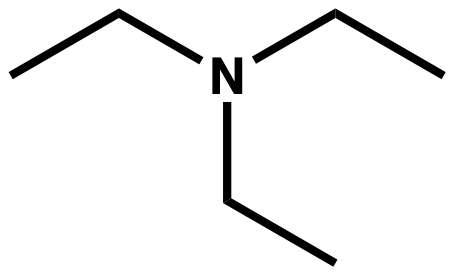
\includegraphics[width=0.75in]{Chapters/Background/Figs/triethyl_amine.png} \\
         CC1=CC(CCC1)Br & 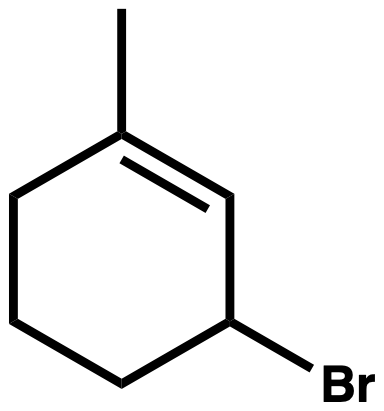
\includegraphics[width=0.7in]{Chapters/Background/Figs/cyclic.png} \\
         \hline
    \end{tabular}
    \caption{Demonstration of the SMILES language}
    \label{table:smiles}
\end{center}
\end{table}

SMILES strings can be imported by most molecule editors for conversion back into two-dimensional drawings or three-dimensional models of the molecules.

\begin{figure}[!h]
    \centering
    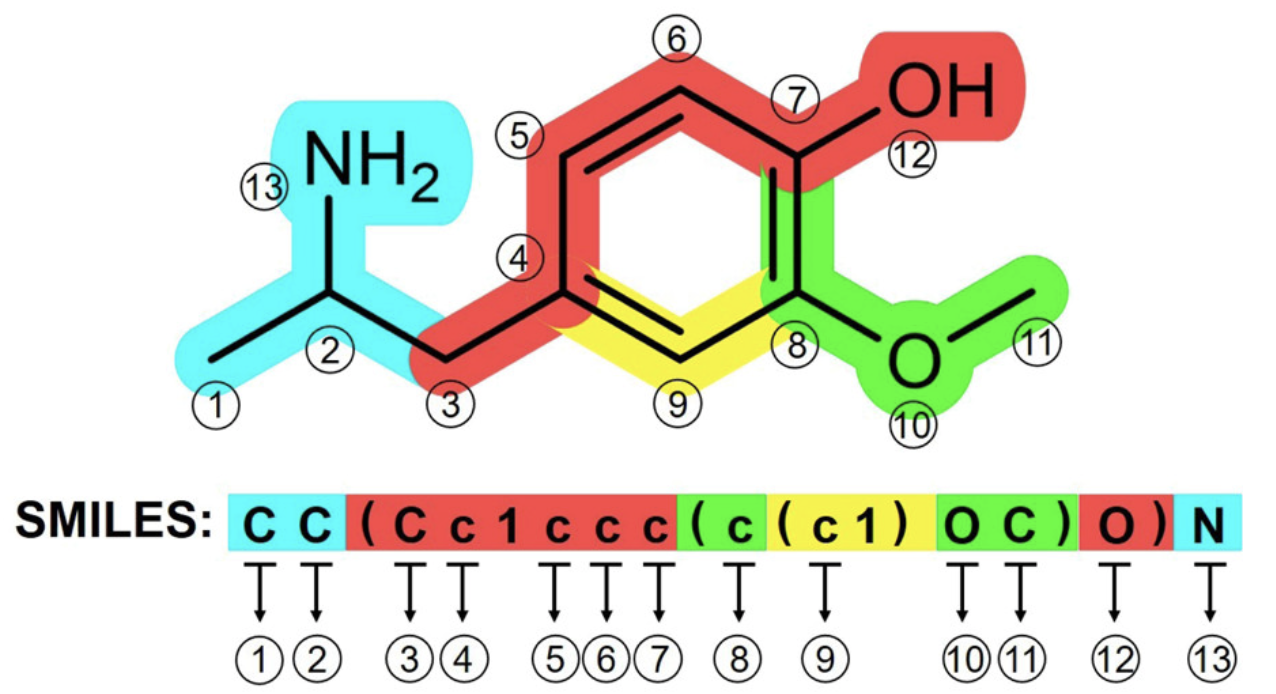
\includegraphics[width=0.8\textwidth]{Chapters/Background/Figs/smiles.png}
    \caption{\label{fig:smiles} \textbf{Illustration of the mapping from chemical structure to SMILES.} Adapted from \cite{Kim2021GenerativeCT}.}
\end{figure}

While SMILES is by far the most widely used text-based representation of molecules, other representations have been developed and are in use to address some shortcomings in SMILES. For example, the International Chemical Identifier (InChI) \cite{Heller2013InChI} string representation, which has a hierarchical construction for specifying tautomeric/stereochemical/charge states, allows greater precision and flexibility in querying molecules from large chemical databases. Another example is Self-referencing embedded strings (SELFIES) \cite{Krenn2020Selfies} which is constructed such that every SELFIES string, including random combinations of characters, is a valid molecule. This property is useful for the application of ML models that generate text as output - using SELFIES as the molecular representation, the model always output valid molecules whereas with SMILES that is not guaranteed.

\subsection{SMARTS}

SMILES arbitrary target specification (SMARTS) is a language for specifying substructural patterns in molecules. The SMARTS line notation is expressive and allows extremely precise and transparent substructural specification and atom typing. % TODO - from wikipedia, update

SMARTS is a line notation for specification of substructural patterns in molecules. While it uses many of the same symbols as SMILES, it also allows specification of wildcard atoms and bonds, which can be used to define substructural queries for chemical database searching. One common misconception is that SMARTS-based substructural searching involves matching of SMILES and SMARTS strings. In fact, both SMILES and SMARTS strings are first converted to internal graph representations which are searched for subgraph isomorphism.

\begin{table}[!h]
    \begin{center}
        \begin{tabular}{|c|c|}
        \hline
             SMARTS & Substructure \\
             \hline
             C & CH\textsubscript{4} \\
             \lbrack Fe2+\rbrack & Fe\textsuperscript{2+} \\
             C=O & CH\textsubscript{2}O \\
             C\#N & HCN (cyan) \\
             CCN(CC)CC & 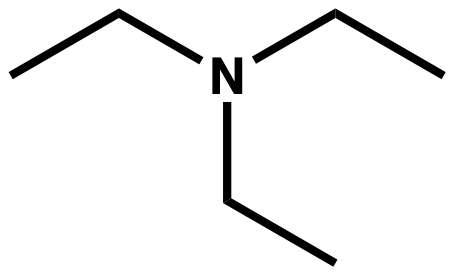
\includegraphics[width=0.75in]{Chapters/Background/Figs/triethyl_amine.png} \\
             CC1=CC(CCC1)Br & 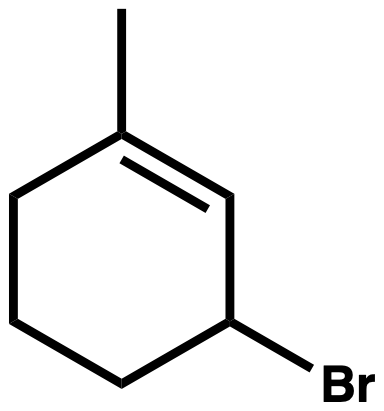
\includegraphics[width=0.7in]{Chapters/Background/Figs/cyclic.png} \\
             \hline
        \end{tabular}
        \caption{Demonstration of the SMILES language}
        \label{table:smarts}
    \end{center}
\end{table}

Chemical substructures. Scaffolds. Reaction templates.

%TODO - example applications from wikidia
The precise and transparent substructural specification that SMARTS allows has been exploited in a number of applications.

Substructural filters defined in SMARTS have been used [7] to identify undesirable compounds when performing strategic pooling of compounds for high-throughput screening. The REOS (rapid elimination of swill) [8] procedure uses SMARTS to filter out reactive, toxic and otherwise undesirable moieties from databases of chemical structures.

RECAP [9](Retrosynthetic Combinatorial Analysis Procedure) uses SMARTS to define bond types. RECAP is a molecule editor which generates fragments of structures by breaking bonds of defined types and the original link points in these are specified using isotopic labels. Searching databases of biologically active compounds for occurrences of fragments allows privileged structural motifs to be identified. The Molecular Slicer [10] is similar to RECAP and has been used to identify fragments that are commonly found in marketed oral drugs.

The Leatherface program[11] is a general purpose molecule editor which allows automated modification of a number of substructural features of molecules in databases, including protonation state, hydrogen count, formal charge, isotopic weight and bond order. The molecular editing rules used by Leatherface are defined in SMARTS. Leatherface can be used to standardise tautomeric and ionization states and to set and enumerate these in preparation of databases[12] for virtual screening. Leatherface has been used in Matched molecular pair analysis, which enables the effects of structural changes (e.g. substitution of hydrogen with chlorine) to be quantified,[13] over a range of structural types.
ALADDIN[14] is a pharmacophore matching program that uses SMARTS to define recognition points (e.g. neutral hydrogen bond acceptor) of pharmacophores. A key problem in pharmacophore matching is that functional groups that are likely to be ionised at physiological pH are typically registered in their neutral forms in structural databases. The ROCS shape matching program allows atom types to be defined using SMARTS.[15]

% Often it is not necessary to fully simulate and understand a chemical reaction and it is sufficient to know the outcome i.e. the major product of it. This is most often the case when experimental organic chemists are willing to validate their synthetic route or when a synthesis planning software uses a reaction prediction model to score its suggestions. This is what is more traditionally referred to as reaction prediction. In these use cases a general purpose model that is able to predict a wide variety of organic reactions with good accuracy is desired. Trained organic chemists usually rationalize reactions based on the reaction mechanisms \cite{Clayden2012}. These mechanisms can be used to categorize organic reactions and each of these categories can be summarised with the help of so called reaction templates. Figure~\ref{fig:rx_template} shows a typical general reaction template for the synthesis of an amide using acid chloride and an amine. Here the $R_1$ and $R_2$ represent any chemical structures. 
% \begin{figure}[htbp!] 
% \centering    
% 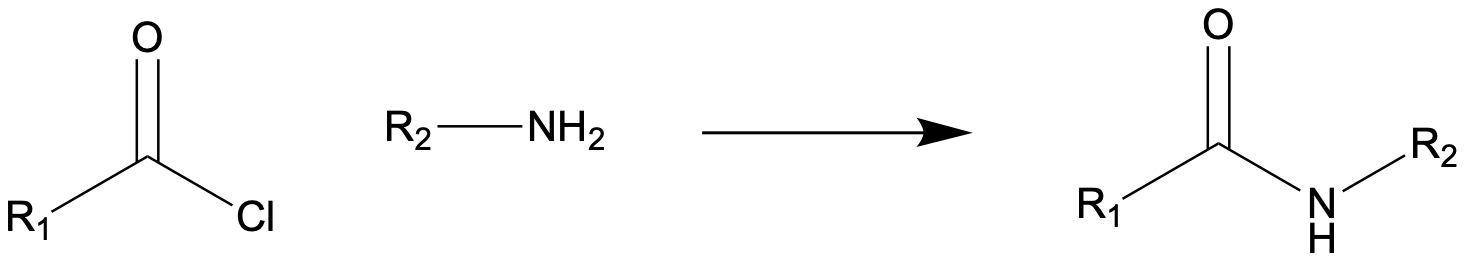
\includegraphics[width=0.75\textwidth]{Chapter2/Figs/Raster/rx_template.png}
% \caption[Reaction template]{An example of a reaction template for the synthesis of an amide}
% \label{fig:rx_template}
% \end{figure}
% These templates can be used for organic reaction prediction by building a catalogue of templates of as many organic reactions as possible. Then given some reactants and reagents as labelled graphs the problem of reaction prediction is transformed into one of subgraph searching to find the best matching general template in the catalogue. When that template is found it can be applied on the input to obtain the predicted outcome of the reaction. This approach was originally proposed and pioneered in the 1980s by E. J. Corey when he used templates for the reverse problem of retrosynthesis \cite{Corey1985Computer-assistedSynthesis}. The template-based approach had some success in forward reaction prediction for example as described in Ref~\cite{Klucznik2018EfficientLaboratory} a template-based model helped design synthetic pathways to a diverse set of 8 drug-like molecules. This method had considerably more success  in retrosynthesis though where there does not exist a single correct solution. One of the major limitation of template-based approaches when applied to forward prediction is scalability, meaning that the template library needs to be maintained and every time a new reaction is reported the associated template needs to be added to the template library. A further problem is that it is often not obvious which parts of the molecule are crucial for a given reaction. This means that given a reaction one can derive a smaller more general template or a larger one that is more specific for the particular reaction. This results in either too many templates matching a particular input resulting in many equally possible reaction outcomes or in the case of larger more specific templates the library will grow very big which results in very slow predictions.  \par

\subsection{Pharmacophores}

A pharmacophore is an abstract description of molecular features that are necessary for molecular recognition of a ligand by a biological macromolecule. IUPAC defines a pharmacophore to be "an ensemble of steric and electronic features that is necessary to ensure the optimal supramolecular interactions with a specific biological target and to trigger (or block) its biological response".[1] A pharmacophore model explains how structurally diverse ligands can bind to a common receptor site. Furthermore, pharmacophore models can be used to identify through de novo design or virtual screening novel ligands that will bind to the same receptor.

Typical pharmacophore features include hydrophobic centroids, aromatic rings, hydrogen bond acceptors or donors, cations, and anions. These pharmacophoric points may be located on the ligand itself or may be projected points presumed to be located in the receptor.

In modern computational chemistry, pharmacophores are used to define the essential features of one or more molecules with the same biological activity. A database of diverse chemical compounds can then be searched for more molecules which share the same features arranged in the same relative orientation. Pharmacophores are also used as the starting point for developing 3D-QSAR models. Such tools and a related concept of "privileged structures", which are "defined as molecular frameworks which are able of providing useful ligands for more than one type of receptor or enzyme target by judicious structural modifications",[3] aid in drug discovery.[4]

Use SMARTS to define pharmacophores.
\subsection{Fingerprints}

The similarity-based[4] virtual screening (a kind of ligand-based virtual screening) assumes that all compounds in a database that are similar to a query compound have similar biological activity. Although this hypothesis is not always valid,[5] quite often the set of retrieved compounds is considerably enriched with actives.[6] To achieve high efficacy of similarity-based screening of databases containing millions of compounds, molecular structures are usually represented by molecular screens (structural keys) or by fixed-size or variable-size molecular fingerprints. Molecular screens and fingerprints can contain both 2D- and 3D-information. However, the 2D-fingerprints, which are a kind of binary fragment descriptors, dominate in this area. Fragment-based structural keys, like MDL keys,[7] are sufficiently good for handling small and medium-sized chemical databases, whereas processing of large databases is performed with fingerprints having much higher information density. Fragment-based Daylight,[8] BCI,[9] and UNITY 2D (Tripos[10]) fingerprints are the best known examples. The most popular similarity measure for comparing chemical structures represented by means of fingerprints is the Tanimoto (or Jaccard) coefficient T. Two structures are usually considered similar if T > 0.85 (for Daylight fingerprints). However, it is a common misunderstanding that a similarity of T > 0.85 reflects similar bioactivities in general ("the 0.85 myth").[11]

Tanimoto similarity.

\section{Computational Approaches}

\subsection{Docking}

In the field of molecular modeling, docking is a method which predicts the preferred orientation of one molecule to a second when a ligand and a target are bound to each other to form a stable complex.[1] Knowledge of the preferred orientation in turn may be used to predict the strength of association or binding affinity between two molecules using, for example, scoring functions.

Schematic illustration of docking a small molecule ligand (green) to a protein target (black) producing a stable complex.
0:13
Docking of a small molecule (green) into the crystal structure of the beta-2 adrenergic G-protein coupled receptor (PDB: 3SN6)
The associations between biologically relevant molecules such as proteins, peptides, nucleic acids, carbohydrates, and lipids play a central role in signal transduction. Furthermore, the relative orientation of the two interacting partners may affect the type of signal produced (e.g., agonism vs antagonism). Therefore, docking is useful for predicting both the strength and type of signal produced.
Molecular docking is one of the most frequently used methods in structure-based drug design, due to its ability to predict the binding-conformation of small molecule ligands to the appropriate target binding site. Characterisation of the binding behaviour plays an important role in rational design of drugs as well as to elucidate fundamental biochemical processes.[2][3]

One can think of molecular docking as a problem of “lock-and-key”, in which one wants to find the correct relative orientation of the “key” which will open up the “lock” (where on the surface of the lock is the key hole, which direction to turn the key after it is inserted, etc.). Here, the protein can be thought of as the “lock” and the ligand can be thought of as a “key”. Molecular docking may be defined as an optimization problem, which would describe the “best-fit” orientation of a ligand that binds to a particular protein of interest. However, since both the ligand and the protein are flexible, a “hand-in-glove” analogy is more appropriate than “lock-and-key”.[4] During the course of the docking process, the ligand and the protein adjust their conformation to achieve an overall "best-fit" and this kind of conformational adjustment resulting in the overall binding is referred to as "induced-fit".[5]
Molecular docking research focuses on computationally simulating the molecular recognition process. It aims to achieve an optimized conformation for both the protein and ligand and relative orientation between protein and ligand such that the free energy of the overall system is minimized.

To perform a docking screen, the first requirement is a structure of the protein of interest. Usually the structure has been determined using a biophysical technique such as X-ray crystallography, NMR spectroscopy or cryo-electron microscopy (cryo-EM), but can also derive from homology modeling construction. This protein structure and a database of potential ligands serve as inputs to a docking program. The success of a docking program depends on two components: the search algorithm and the scoring function.
Search algorithm[edit]
Main article: Searching the conformational space for docking
The search space in theory consists of all possible orientations and conformations of the protein paired with the ligand. However, in practice with current computational resources, it is impossible to exhaustively explore the search space — this would involve enumerating all possible distortions of each molecule (molecules are dynamic and exist in an ensemble of conformational states) and all possible rotational and translational orientations of the ligand relative to the protein at a given level of granularity. Most docking programs in use account for the whole conformational space of the ligand (flexible ligand), and several attempt to model a flexible protein receptor. Each "snapshot" of the pair is referred to as a pose.
A variety of conformational search strategies have been applied to the ligand and to the receptor. These include:
systematic or stochastic torsional searches about rotatable bonds
molecular dynamics simulations
genetic algorithms to "evolve" new low energy conformations and where the score of each pose acts as the fitness function used to select individuals for the next iteration.

Ligand flexibility[edit]
Conformations of the ligand may be generated in the absence of the receptor and subsequently docked[14] or conformations may be generated on-the-fly in the presence of the receptor binding cavity,[15] or with full rotational flexibility of every dihedral angle using fragment based docking.[16] Force field energy evaluation are most often used to select energetically reasonable conformations,[17] but knowledge-based methods have also been used.[18]
Peptides are both highly flexible and relatively large-sized molecules, which makes modeling their flexibility a challenging task. A number of methods were developed to allow for efficient modeling of flexibility of peptides during protein-peptide docking.[19]
Receptor flexibility[edit]
Computational capacity has increased dramatically over the last decade making possible the use of more sophisticated and computationally intensive methods in computer-assisted drug design. However, dealing with receptor flexibility in docking methodologies is still a thorny issue.[20] The main reason behind this difficulty is the large number of degrees of freedom that have to be considered in this kind of calculations. Neglecting it, however, in some of the cases may lead to poor docking results in terms of binding pose prediction.[21]
Multiple static structures experimentally determined for the same protein in different conformations are often used to emulate receptor flexibility.[22] Alternatively rotamer libraries of amino acid side chains that surround the binding cavity may be searched to generate alternate but energetically reasonable protein conformations.[23][24]
Scoring function[edit]
Main article: Scoring functions for docking
Docking programs generate a large number of potential ligand poses, of which some can be immediately rejected due to clashes with the protein. The remainder are evaluated using some scoring function, which takes a pose as input and returns a number indicating the likelihood that the pose represents a favorable binding interaction and ranks one ligand relative to another.
Most scoring functions are physics-based molecular mechanics force fields that estimate the energy of the pose within the binding site. The various contributions to binding can be written as an additive equation:

% {\displaystyle \bigtriangleup G_{bind}=\bigtriangleup G_{solvent}+\bigtriangleup G_{conf}+\bigtriangleup G_{int}+\bigtriangleup G_{rot}+\bigtriangleup G_{t/t}+\bigtriangleup G_{vib}}
The components consist of solvent effects, conformational changes in the protein and ligand, free energy due to protein-ligand interactions, internal rotations, association energy of ligand and receptor to form a single complex and free energy due to changes in vibrational modes.[25] A low (negative) energy indicates a stable system and thus a likely binding interaction.
Alternative approaches use modified scoring functions to include constraints based on known key protein-ligand interactions,[26] or knowledge-based potentials derived from interactions observed in large databases of protein-ligand structures (e.g. the Protein Data Bank).[27]
There are a large number of structures from X-ray crystallography for complexes between proteins and high affinity ligands, but comparatively fewer for low affinity ligands as the latter complexes tend to be less stable and therefore more difficult to crystallize. Scoring functions trained with this data can dock high affinity ligands correctly, but they will also give plausible docked conformations for ligands that do not bind. This gives a large number of false positive hits, i.e., ligands predicted to bind to the protein that actually don't when placed together in a test tube.
One way to reduce the number of false positives is to recalculate the energy of the top scoring poses using (potentially) more accurate but computationally more intensive techniques such as Generalized Born or Poisson-Boltzmann methods.[9]

Simulating the docking process is much more complicated. In this approach, the protein and the ligand are separated by some physical distance, and the ligand finds its position into the protein's active site after a certain number of “moves” in its conformational space. The moves incorporate rigid body transformations such as translations and rotations, as well as internal changes to the ligand's structure including torsion angle rotations. Each of these moves in the conformation space of the ligand induces a total energetic cost of the system. Hence, the system's total energy is calculated after every move.
The obvious advantage of docking simulation is that ligand flexibility is easily incorporated, whereas shape complementarity techniques must use ingenious methods to incorporate flexibility in ligands. Also, it more accurately models reality, whereas shape complementary techniques are more of an abstraction.
Clearly, simulation is computationally expensive, having to explore a large energy landscape. Grid-based techniques, optimization methods, and increased computer speed have made docking simulation more realistic.

Docking assessment[edit]
See also: Critical Assessment of Prediction of Interactions
The interdependence between sampling and scoring function affects the docking capability in predicting plausible poses or binding affinities for novel compounds. Thus, an assessment of a docking protocol is generally required (when experimental data is available) to determine its predictive capability. Docking assessment can be performed using different strategies, such as:
docking accuracy (DA) calculation;
the correlation between a docking score and the experimental response or determination of the enrichment factor (EF);[28]
the distance between an ion-binding moiety and the ion in the active site;
the presence of induce-fit models.
Docking accuracy[edit]
Docking accuracy[29][30] represents one measure to quantify the fitness of a docking program by rationalizing the ability to predict the right pose of a ligand with respect to that experimentally observed.[31]
Enrichment factor[edit]
Docking screens can also be evaluated by the enrichment of annotated ligands of known binders from among a large database of presumed non-binding, “decoy” molecules.[28] In this way, the success of a docking screen is evaluated by its capacity to enrich the small number of known active compounds in the top ranks of a screen from among a much greater number of decoy molecules in the database. The area under the receiver operating characteristic (ROC) curve is widely used to evaluate its performance.
Prospective[edit]
Resulting hits from docking screens are subjected to pharmacological validation (e.g. IC50, affinity or potency measurements). Only prospective studies constitute conclusive proof of the suitability of a technique for a particular target.[32] In the case of G protein-coupled receptors (GPCRs), which are targets of more than 30% of marketed drugs, molecular docking led to the discovery of more than 500 GPCR ligands.[33]
Benchmarking[edit]
The potential of docking programs to reproduce binding modes as determined by X-ray crystallography can be assessed by a range of docking benchmark sets.
For small molecules, several benchmark data sets for docking and virtual screening exist e.g. Astex Diverse Set consisting of high quality protein-ligand X-ray crystal structures[34] or the Directory of Useful Decoys (DUD) for evaluation of virtual screening performance.[28]
An evaluation of docking programs for their potential to reproduce peptide binding modes can be assessed by Lessons for Efficiency Assessment of Docking and Scoring (LEADS-PEP).[35]
Applications[edit]
A binding interaction between a small molecule ligand and an enzyme protein may result in activation or inhibition of the enzyme. If the protein is a receptor, ligand binding may result in agonism or antagonism. Docking is most commonly used in the field of drug design — most drugs are small organic molecules, and docking may be applied to:
hit identification – docking combined with a scoring function can be used to quickly screen large databases of potential drugs in silico to identify molecules that are likely to bind to protein target of interest (see virtual screening). Reverse pharmacology routinely uses docking for target identification.
lead optimization – docking can be used to predict in where and in which relative orientation a ligand binds to a protein (also referred to as the binding mode or pose). This information may in turn be used to design more potent and selective analogs.
bioremediation – protein ligand docking can also be used to predict pollutants that can be degraded by enzymes.[36][37]

Theory. Virtual screening. Virtual library?

In contrast to high-throughput screening, virtual screening involves computationally screening in silico libraries of compounds, by means of various methods such as docking, to identify members likely to possess desired properties such as biological activity against a given target. In some cases, combinatorial chemistry is used in the development of the library to increase the efficiency in mining the chemical space. More commonly, a diverse library of small molecules or natural products is screened.

\subsection{FEP?}

\section{Machine Learning}

\subsection{Random Forest}

Random forests or random decision forests is an ensemble learning method for classification, regression and other tasks that operates by constructing a multitude of decision trees at training time. For classification tasks, the output of the random forest is the class selected by most trees. For regression tasks, the mean or average prediction of the individual trees is returned.[1][2] Random decision forests correct for decision trees' habit of overfitting to their training set.[3]:587–588 Random forests generally outperform decision trees, but their accuracy is lower than gradient boosted trees.[citation needed] However, data characteristics can affect their performance.[4][5]

Random Forests are a decision tree-based model that use an ensemble of multiple weak regressors to make predictions [47]. Each tree is constructed to find a series of decision boundaries that split the data to minimise the squared deviations between the samples and the sample mean in each branch or leaf of the tree. Predictions are made by averaging the outputs of the different trees when applied to new data. To overcome issues of over-fitting common to decision tree methods, Random Forests use bagging and random subspace projection to reduce the correlation between the trees, improving their generalisation performance.

Examples of RF with morgan fingerprints.
\subsection{Deep Learning}

In contrast to shallow learning, the deep learning revolution of the last decade is built around models that learn their representations from raw data inputs. The workhorse of deep learning is the neural network. At their heart, neural networks are compositions of feature maps that transform the raw input features, x, into a new set of features that are linearly related to their target, y. The prototypical example of a neural network is the multi-layer perceptron (MLP). A l-layer MLP approximates functions f(x) using l successive non-linear feature maps constructed as compositions of affine transformations and non linearities, i.e.

Neural Networks. Loss functions. Optimisation.

\begin{equation}
    y = f(x, \theta)
\end{equation}

\begin{equation}
    \hat{theta} = \arg\min_{\theta} \mathcal{L}(\theta)
\end{equation}

\begin{equation}
    \hat{y} = \sigma(\mathbf{W} \cdot \mathbf{x} + \mathbf{b})
\end{equation}

\begin{equation}
    \mathcal{L}(y, \hat{y}) = \sum_{i}(y_i - \hat{y}_i)^{2}
\end{equation}

The remarkable success of deep learning emerges from the fact that neural networks, such as MLPs, can be optimised effectively using first-order gradient-based approaches. Moreover, the necessary gradients can be efficiently calculated using the chain rule by back- propagation of the training loss. In practice, modern neural networks are implemented inside automatic differentiation frameworks that abstract away the technical burden of implementing back-propagation [71, 72]. In addition, these frameworks are designed to enable the necessary calculations to be carried out on hardware accelerators, such as graphical processing units (GPUs), that dramatically reduce the time for training.
The most simple gradient-based optimisation algorithm is gradient-descent. In gradient descent at each step the model’s parameters are updated according to

\begin{equation}
    \theta_{t+1} = \theta_t - \eta \nabla_{\theta} \mathcal{L}
\end{equation}

where the learning rate, $\eta$, is a hyper-parameter of the optimiser that determines the size of the parameter updates. In practice, the full-batch gradient of the loss, $\nabla_{\theta}\mathcal{L}(\theta_{t})$ is replaced with a stochastic approximation of the gradient calculated on a mini-batch of data randomly sampled from all the available training data. Typically mini-batches are randomly drawn from the training data without replacement until all the training examples have been considered. Each complete cycle through the training set is referred to as an epoch. After each epoch, the training set is shuffled and the process is repeated until the loss has satisfactorily converged. Replacing full-batch gradient descent with mini-batch stochastic gradient descent significantly speeds up optimisation, reducing the amount of computation required to determine the gradient for each step and providing helpful regularisation effects that drive the optimisation towards flatter local basins of attraction in the loss landscape. Further improvements to model optimisation procedures can be achieved by incorporating additional terms such as momentum, learning rate schedules, or adaptive learning rates [73], and additional regularisation procedures such as weight decay, early-stopping, or dropout [74].

In the above description of the MLP, the key requirement is that the model is end- to-end differentiable. This allows the parameters of the model to be optimised by the combination of back-propagation and gradient descent. Accordingly, provided we ensure that all operations in our models have defined derivatives, we can build up novel neural networks architectures with specific inductive biases as compositions of custom differentiable building blocks – notable examples are recurrent neural networks (RNNs) that are designed to handle series data (e.g. Gated-Recurrent-Unit (GRU) [75] and Long-Short-Term-Memory (LSTM) networks [76]) and convolutional neural networks
(CNNs) that build in translational invariance for computer vision applications (e.g. LeNet [77], AlexNet [78], and ResNets [79]).

Within materials science, this ability to compose differentiable building blocks into novel architectures has led to the development of a wide variety of message-passing neural networks that operate directly on the atomic coordinates of molecules and materials. Typically these models operate on “radius”-graphs of interconnected local environments determined using a cutoff radius – the resulting data structure closely mirrors that of Verlet lists used in atomistic simulations [80]. The nodes of the graphs encode atoms with edges encoding interactions or bonds. As with shallow descriptor-based models, it is important to encode the underlying symmetries of the problem into the network architecture. Earlier models ensured SO(3)-invariance by only including position information via the relative distances between connected sites [81–83]. More recently SO(3)-equivariant architectures have been proposed that include angular and higher-order information or relative displacement vectors between atoms to allow construction of message passing operations that maintain equivariance [84].



Examples of NNs with fingerprints and SMILES.

\subsection{Evaluating Models}

ROC-AUC. Accuracy. Enrichment.

%TODO - from wikipedia
A receiver operating characteristic curve, or ROC curve, is a graphical plot that illustrates the diagnostic ability of a binary classifier system as its discrimination threshold is varied.

The ROC curve is created by plotting the true positive rate (TPR) against the false positive rate (FPR) at various threshold settings. The true-positive rate is also known as sensitivity, recall or probability of detection.[10] The false-positive rate is also known as probability of false alarm[10] and can be calculated as (1 - specificity).

\begin{equation}
    \mathrm{EF}(n) = \frac{\mathrm{Hit\: rate (predicted\: top - }n)}{\mathrm{Hit\: rate (baseline)}}
\end{equation}


Train-Test splitting

Random split, scaffold split, time split

In machine learning, a common task is the study and construction of algorithms that can learn from and make predictions on data.[1] Such algorithms function by making data-driven predictions or decisions,[2] through building a mathematical model from input data. These input data used to build the model are usually divided in multiple data sets. In particular, three data sets are commonly used in different stages of the creation of the model: training, validation and test sets.
The model is initially fit on a training data set,[3] which is a set of examples used to fit the parameters (e.g. weights of connections between neurons in artificial neural networks) of the model.[4] The model (e.g. a naive Bayes classifier) is trained on the training data set using a supervised learning method, for example using optimization methods such as gradient descent or stochastic gradient descent. In practice, the training data set often consists of pairs of an input vector (or scalar) and the corresponding output vector (or scalar), where the answer key is commonly denoted as the target (or label). The current model is run with the training data set and produces a result, which is then compared with the target, for each input vector in the training data set. Based on the result of the comparison and the specific learning algorithm being used, the parameters of the model are adjusted. The model fitting can include both variable selection and parameter estimation.
Successively, the fitted model is used to predict the responses for the observations in a second data set called the validation data set.[3] The validation data set provides an unbiased evaluation of a model fit on the training data set while tuning the model's hyperparameters[5] (e.g. the number of hidden units—layers and layer widths—in a neural network[4]). Validation datasets can be used for regularization by early stopping (stopping training when the error on the validation data set increases, as this is a sign of over-fitting to the training data set).[6] This simple procedure is complicated in practice by the fact that the validation dataset's error may fluctuate during training, producing multiple local minima. This complication has led to the creation of many ad-hoc rules for deciding when over-fitting has truly begun.[6]
Finally, the test data set is a data set used to provide an unbiased evaluation of a final model fit on the training data set.[5] If the data in the test data set has never been used in training (for example in cross-validation), the test data set is also called a holdout data set. The term "validation set" is sometimes used instead of "test set" in some literature (e.g., if the original data set was partitioned into only two subsets, the test set might be referred to as the validation set).[5]
Deciding the sizes and strategies for data set division in training, test and validation sets is very dependent on the problem and data available.[7]

\section{Applications of ML on Drug Discovery}

\subsection{QSAR}

\subsection{Reaction Prediction}

Note on bioactivity?

% In the paper of Nam and Kim \cite{Nam2016LinkingReactions} they formulated the reaction prediction problem as a translation task. The input SMILES corresponding to the reactant and reagent molecules are tokenized, so that each character of SMILES is equivalent to a word and the whole input is equivalent to a sentence. This sentence is than ``translated" by the model to the product SMILES. Neural machine translation models are trained using a large parallel corpus. This is available in the case of organic reactions from patents and publications or can be generated using templates of elementary reactions. The method of Nam and Kim served as an important proof of concept but could not match the accuracy of rule-based and graph-to-graph models. \par
% %The method was built on a neural network building block called gated recurrent unit (GRU) \cite{Cho2014LearningTranslation}. GRUs are a type of recurrent neural networks that process arbitrarily long inputs token by token, so that the hidden state representation of each token depends on the previous ones. %The model used in the paper is illustrated on Figure~\ref{fig:gru}. 
% %This model served as a proof-of-concept but could not match the accuracy of graph-to-graph and template based approaches. \par

% \iffalse
% \begin{figure}[htbp!] 
% \centering    
% \includegraphics[width=0.9\textwidth]{Chapter2/Figs/Raster/gru.png}
% \caption[GRU for reaction predictions]{The architecture used by Nam and Kim. The input SMILES string is tokenized into ``words", each token is embedded using a learnt embedding and processed by a three layer GRU network. The product is generated using attention mechanism.}
% \label{fig:gru}
% \end{figure}
% \fi

% The large breakthrough of sequence-to-sequence models for reaction prediction came after the introduction of a new and innovative architecture for neural machine translation by Vaswani et. al. \cite{Vaswani2017}. The so called Transformer model revolutionized the entire industry of machine translation and found use in many other areas of machine learning ever since. In the next section the Transformer architecture is described in detail followed by a discussion of the Molecular Transformer. 

% \section{The Molecular Transformer}

% \subsection{The Transformer architecture}

% The Transformer architecture was originally developed for machine translation tasks. It has an encoder-decoder structure. Both the encoder and the decoder are made up of so called transformer blocks that process the inputs by applying a multi-head scaled dot-product attention mechanism followed by layer normalization and some fully connected feed forward layers. In the following each part is described in detail. 

% \subsubsection{Encoder}
% The input to the model is a sentence made up of different words that are contained in a vocabulary. Each word in the vocabulary has a learnt fixed-length vector representation. Passing these vectors to the model would not be enough though as these vectors have no reference to where the given word appears inside the sequence. To encode this information as well another vector of the same length is added to each word-vector that depends on the position inside the sequence: \par

% \begin{equation}
%     PE_{(pos, 2i)}=\sin(pos/10000^{2i/d_{model}})
% \end{equation}
% \begin{equation}
%     PE_{(pos, 2i+1)}=\cos(pos/10000^{2i/d_{model}})
% \end{equation}

% This vector representation of the input text is passed into the transformer blocks. These consist of a multi-head attention layer with residual connection \cite{He2016DeepRecognition} followed by layer normalization \cite{Ba2016LayerNormalization} and a 2-layer fully connected feed forward neural network with ReLU activation. The encoder of the model is made up of $N=6$ transformer blocks as illustrated on Figure~\ref{fig:transformer}

% \begin{figure}[ht]
% \centering    
% \includegraphics[width=2.9in]{transformer_diagram.png}
% \caption{Graphical illustration of the full transformer model \cite{Vaswani2017}}
% \label{fig:transformer}
% \end{figure}

% \subsubsection{Multi-head scaled dot-product attention}
% The multi-head scaled dot-product attention is the heart of the Transformer model. It is a specific version of a general deep learning technique called attention. Given a set of vector \emph{values} and a vector \emph{query} the attention mechanism computes a weighted sum of the \emph{values} dependent on the \emph{query}. The sum represents a selective summary of the \emph{values} and the \emph{query} determines the importance of each vector, i. e. determines how much each \emph{value} vector is attended to.\par 
% The full attention mechanism operates by performing the following steps. Given some vector values $\bm{h_1}, \bm{h_2},\dots, \bm{h_N} \in \mathbb{R} ^{d_1}$ and a query $\bm{q} \in \mathbb{R} ^{d_2}$ \par

% \begin{enumerate}
%     \item First the attention scores $\bm{e} \in \mathbb{R}^N$ are computed. In the case of the scaled dot-product attention $d_1=d_2$ and $\bm{e}$ is simply defined as the scaled vector of projections $e_i=\frac{\bm{q}^\intercal \bm{h}_i}{\sqrt{d_1}}$
%     \item To generate the attention distribution $\bm{\alpha}$ the softmax of $\bm{e}$ is taken: 
%     \begin{equation}
%         \alpha_i=\frac{\exp{(e_i)}}{\sum_{j=1}^N \exp{(e_j)}} 
%         \label{eqn:softmax}
%     \end{equation}
%     \item Finally the attention distribution is used to take the weighted sum of the values to obtain the final output
%     \begin{equation}
%         \bm{a}=\sum_{i=1}^N \alpha_i \: \bm{h}_i \; \in \mathbb{R}^{d_1}
%     \end{equation}
% \end{enumerate}

% The scaling factor in the dot product serves the purpose of preventing some of the projection becoming overwhelmingly large which in turn would lead to the softmax function being sharply peaked around those values and being shallow everywhere else. This would result in very small gradients at most places that can substantially slow down the training.\par

% In the Transformer encoder the above described attention mechanism is used such that given a set of input vectors a new vector is calculated for all of them (being the query) from the others (being the keys). This is called self-attention. This way during training the model is able to learn which vectors (that are representing words or atoms) usually interact with each other. This interaction can result in a large value in the attention distribution. \par

% Usually the input, be it a chemical formula or a sentence contains a rich structure with the words affecting each others meanings in multiple ways. The problem with the simple self-attention mechanism is that by defining a single attention distribution for each input vector only one way of interaction can be learnt by the model. To give the model more flexibility to potentially learn more complex interaction structures multi-head attention was introduced. This mechanism maps the vectors to $h=8$ different lower dimensional spaces via a set of learnt linear transformations. The self-attention mechanism is than applied in these lower dimensional spaces simultaneously. The outputs of the different attention heads are finally concatenated and fed into a linear neural network layer. The whole mechanism is illustrated on Figure~\ref{fig:multihead_attention}

% \begin{figure}
% \centering    
% \includegraphics[width=2.2in]{mulithead_attention.png}
% \caption{Graphical illustration of the multi-head attention \cite{Vaswani2017}}
% \label{fig:multihead_attention}
% \end{figure}

% \subsubsection{Decoder}

% The outputs of the encoder which are $N$ vectors if the input sequence is $N$ words long are fed into the decoder which has a structure almost identical to the encoder. The first modifications concern the masking in the multi-head self-attention layers to make sure that every token in the output translation can only attend to the preceding ones. The second modification of the attention mechanism is making use of the encoder outputs by using them as keys whilst the queries are the outputs of the previous decoder layer. \par
% The generation of the translation happens in a sequential manner. First the embedding of the special \texttt{<start>} token is fed into the decoder and passed through the layers. The result is projected to a vector that has the same dimensionality as the size of the vocabulary. Finally the softmax function is applied to obtain the probability of the first word. The second word is generated by passing in the first word (and the \texttt{start} token) to the decoder, the third is generated by passing in the first and the second etc. This is called autoregressive translation. Finally the translation terminates either when the most probable next token is the special \texttt{<end>} token or when the maximum sequence length is reached. By multiplying together the next-token probabilities and normalizing with respect to the length of the output a confidence score of the translation can be obtained. 


% \subsubsection{Datasets}
% The first dataset used in this work is the freely available USPTO dataset \cite{Lowe2012} that was filtered by Jin et. al. \cite{Jin2017}. Further filtering was preformed to remove some remaining duplicates or reactions that were erroneously text mined. These included examples such as reactions whose sole product is nitric acid, sulfuric acid, chloride ion etc. This way the final number of reactions in the dataset was 471 791 of which 377 419  were used for training, 23 589 for validation and 70 765 were used as a hold-out test set. The training set was augmented by an equal number of random equivalent SMILES strings. Augmentation can help the model to learn the underlying molecular graph from the SMILES sequence. \par
% The model trained in the way described above achieved 88.8\% Top-1 accuracy on the test set. This model was used throughout the interpretability experiments and is referred to as USPTO Transformer. \par
% The second dataset used was the commercial Pistachio dataset \cite{Mayfield2018Pistachio2.0}. This dataset contains over 9 million reactions text mined from US and EPO patents. This dataset was filtered similarly to USPTO to remove erroneous and duplicate reactions. It turned out that many of the 9 million reactions were duplicates corresponding to different patent IDs. In the end a dataset of 2 375 385 reactions was obtained of which 2 019 078 was used for training, 118 770 for validation and 237 537 for testing. \par
% The model trained as described above achieved 76.4\% Top-1 accuracy on the test set. Even though this looks like a substantially lower performance in reality the two models perform similarly well on new reactions. The possible reasons for the large difference in the measured performance on the held-out test sets are described in detail in Chapter~\ref{chap:interpr_molt}. This model obtained was also used in the interpretability experiments to test the effect of increased training set size on the models understanding of chemistry and is referred to as Pistachio Transformer in the rest of the thesis. \par